\documentclass[a4paper,landscape]{article}

\usepackage[landscape,top=0cm,left=0cm,bottom=0cm,right=0cm]{geometry}
\usepackage{tikz}
\usepackage{background}
\usepackage{blindtext}
\usetikzlibrary{matrix, shapes.misc, calc}

\pagestyle{empty}
\setlength{\parindent}{0cm}
\backgroundsetup{scale = 1, angle = 0, opacity = 1, color=black, contents = {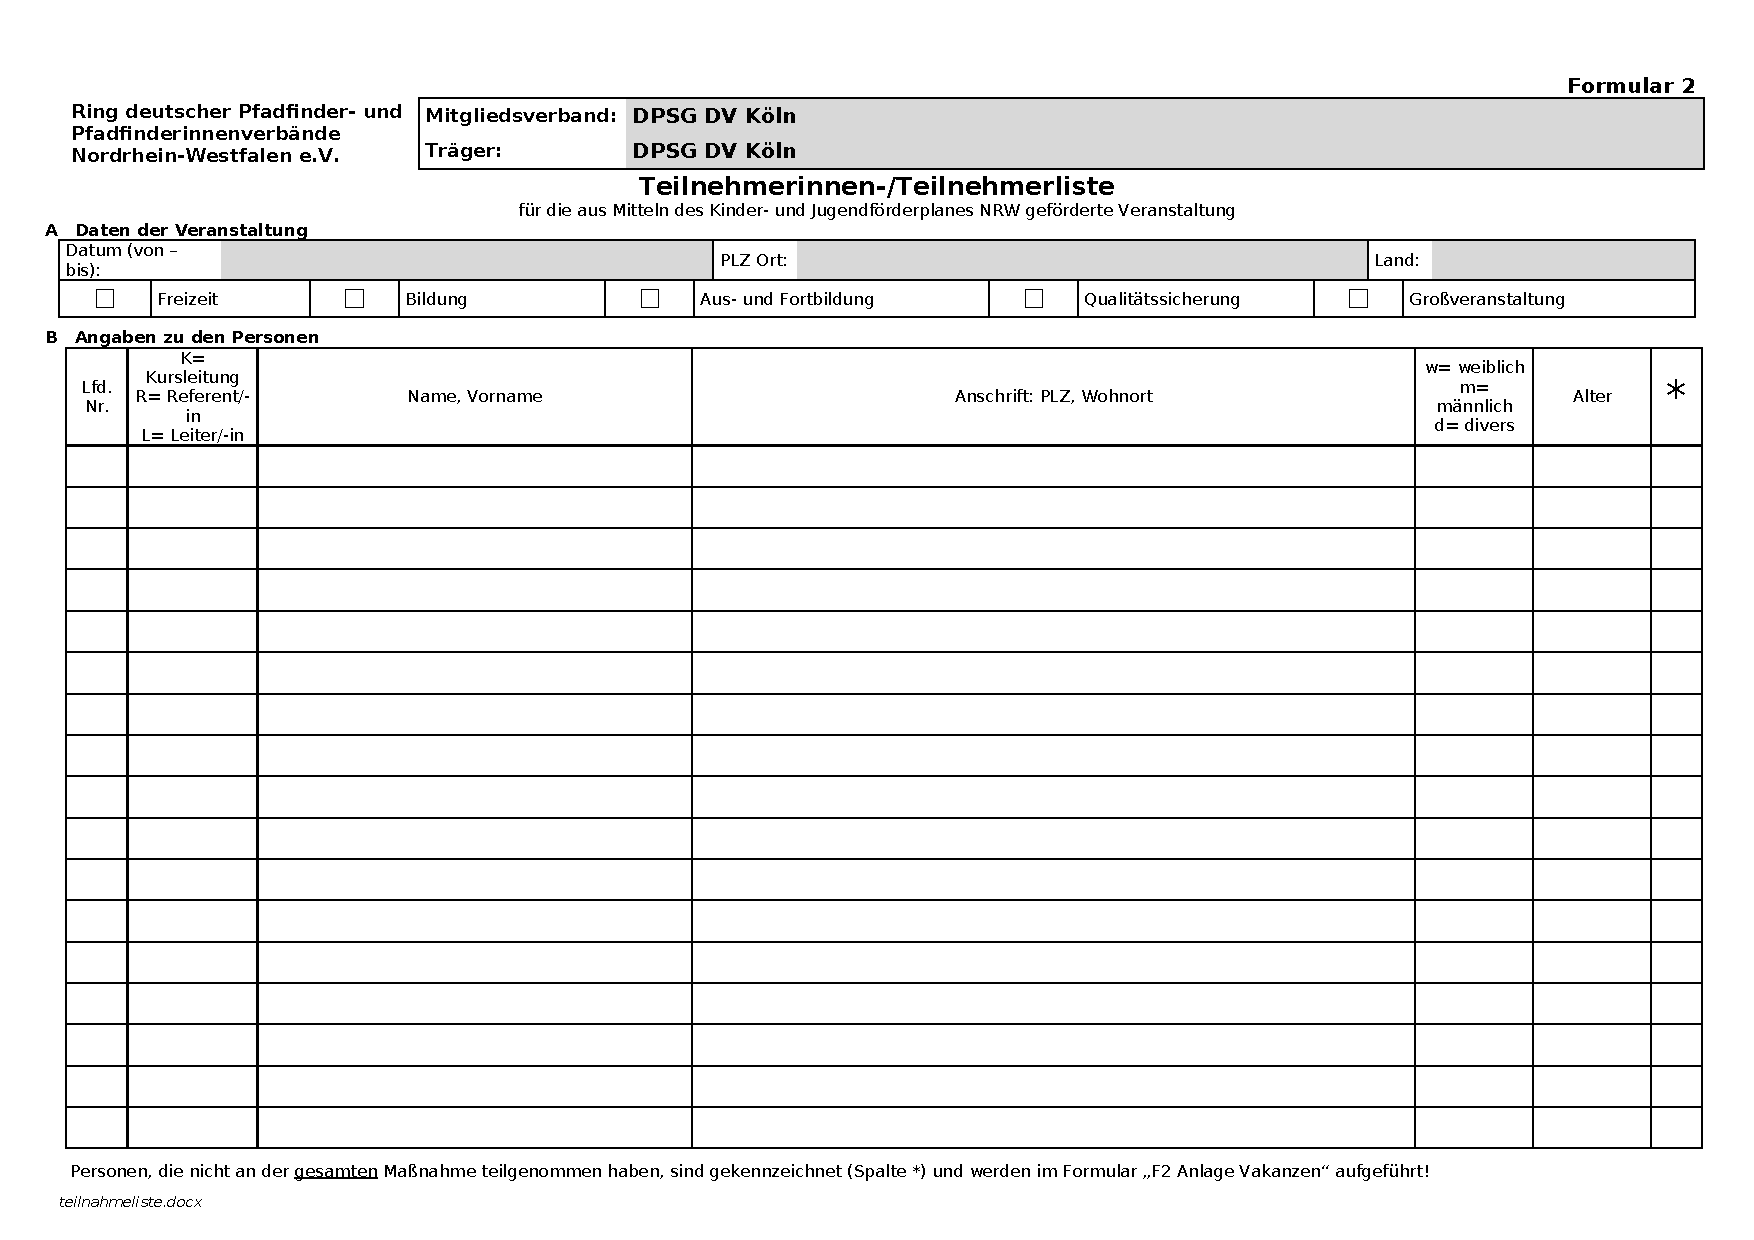
\includegraphics[width = \paperwidth, height = \paperheight] {rdp-nrw.pdf}}}

\begin{document}
\noindent \sffamily

@foreach($members as $chunk)
\begin{tikzpicture}[remember picture,overlay,yscale=-1]
    \node[anchor=base west] at (38mm,41.62mm) {\bfseries{\large{<<<!!$dateRange!!>>>}}};
\node[anchor=base west] at (135.2mm,41.62mm) {\bfseries{\large{<<<!!$zipLocation!!>>>}}};
    \node[anchor=base west] at (242.7mm,41.62mm) {\bfseries{\large{<<<!!$countryName!!>>>}}};

\node[thick, cross out,draw=black,text width=2.4mm, text height=2.4mm, inner sep=0mm] at (17.76mm,47.10mm) {};

@foreach($chunk as $i => $member)
    \node[anchor=base, text width=7.75mm, align=center] at ($(16.35mm, 76.6mm + 7mm * <<<$i % 17>>>)$) {<<<$i+1>>>};
    \node[anchor=base, text width=18mm, align=center] at ($(32.55mm, 76.6mm + 7mm * <<<$i%17>>>)$) {<<<$memberShort($member)>>>};
    \node[anchor=base, text width=70mm, align=center] at ($(80.25mm, 76.6mm + 7mm * <<<$i%17>>>)$) {<<<$memberName($member)>>>};
    \node[anchor=base, text width=118mm, align=center] at ($(178.25mm, 76.6mm + 7mm * <<<$i%17>>>)$) {<<<$memberAddress($member)>>>};
    \node[anchor=base, text width=16mm, align=center] at ($(249.50mm, 76.6mm + 7mm * <<<$i%17>>>)$) {<<<$memberGender($member)>>>};
    \node[anchor=base, text width=16mm, align=center] at ($(269.50mm, 76.6mm + 7mm * <<<$i%17>>>)$) {<<<$memberAge($member)>>>};
@endforeach

\end{tikzpicture}

\pagebreak

@endforeach
\end{document}

